\subsection{Multi-View-Coding}\label{subsec:mvc}

\subsubsection{Räumliche und Zeitliche Nachbarn eines Rahmens}
\begin{wrapfigure}{r}{0.4\textwidth}
    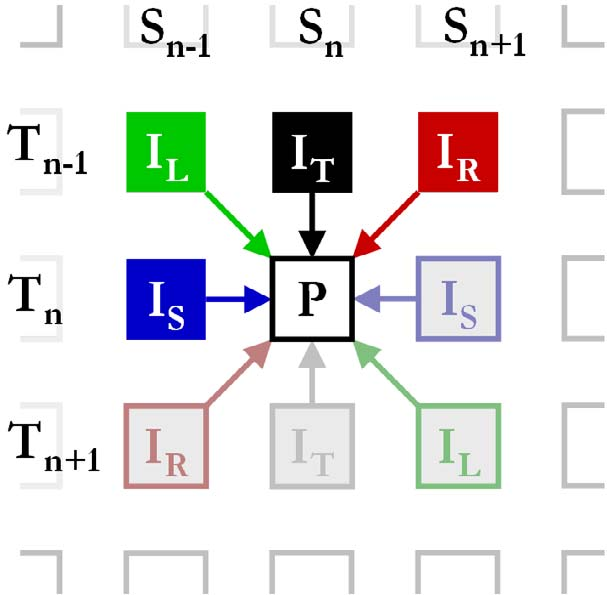
\includegraphics[width=5cm]{../img/prediction}
\end{wrapfigure}

Jeder Rahmen hat drei einzigartige räumliche sowie zeitliche Nachbarn.
Diese bestehen aus dem Rahmen der benachbarten Perspektive, dem vorherigen Rahmen der selben Perspektive, sowie
dem vorherigen Rahmen der benachbarten Perspektive.

\noindent\newline Es stellt sich für uns die Frage, welche der Perspektiven der beste Prädiktor unseres Rahmens ist.
Durch eine statistische Analyse der mehrerer Videosequenzen kann diese Frage beantwortet werden.
Hierzu müssen die Kosten des Erstellens eines P-Rahmens zwischen den Nachbarn verglichen werden.
Zwar gibt es starke Variationen zwischen Videosequenzen, im Durchschnitt ist jedoch der direkte zeitliche Nachbar
der beste Prädiktor.
Gefolgt wird dieser vom direkten räumlichen Nachbarn.
